\section{MATHEMATICAL MODELS IN ELECTROPHYSIOLOGY}

Model the bio-electric cardiac source and the conducting media in order to derive the potential field is known as the \textsl{forward problem of electro-physiology}. There are different mathematical models that can achieve this goal, with more or less accuracy, as we will see in the followings paragraphs. 

\subsection{Cardiac Cells Arrangement Models}

Now we are going to present two mathematical models for the electric potential propagation over the cardiac tissue. For the mesoscopic scale is often used the so called bi-domain model, while for large problems at macroscopic scale the mono-domain model is usually used, mainly due to his computational low cost (in comparison with bi-domain model). The mathematical foundations, like the proof of existence and uniqueness of the solutions where performed by Colli Franzone and Savaré in \cite{colli_franzone}.

As general definitions, let us define $d$ as the dimension of the problem (usually 2 or 3), the domain $\Omega \subset \mathbb{R}^d$, and $\Gamma = \partial \Omega$ such that $\Gamma = \Gamma_D \cup \Gamma_N$ and $\Gamma_D \cap \Gamma_N = \emptyset$. Also, let us define the internal-variable vector that controls the cell membrane recovery (i.e. the action potential model) $\vec{r}: \Omega \times \mathbb{R}^+ \rightarrow \mathbb{R}^m$, where m is the number of parameters used to model the cellular membrane process.

\subsubsection{The Bi-Domain Model}

As far the author knows, the more detailed way to describe the potential propagation through the cardiac tissue is the bi-domain approach. This model establish an equation that describes the cardiac tissue considering the extra and intra cellular potentials separately. Furthermore, every cell membrane is considered as a capacitor, and separately, the resistivity of each ion channel in it (see Figure \ref{fig:bidomain_model}) is also considered. One way to express the anisotropic bi-domain model is trough the \textsl{PP-formulation}, that is enunciated in the next paragraph.

\begin{figure}[H]
\centering
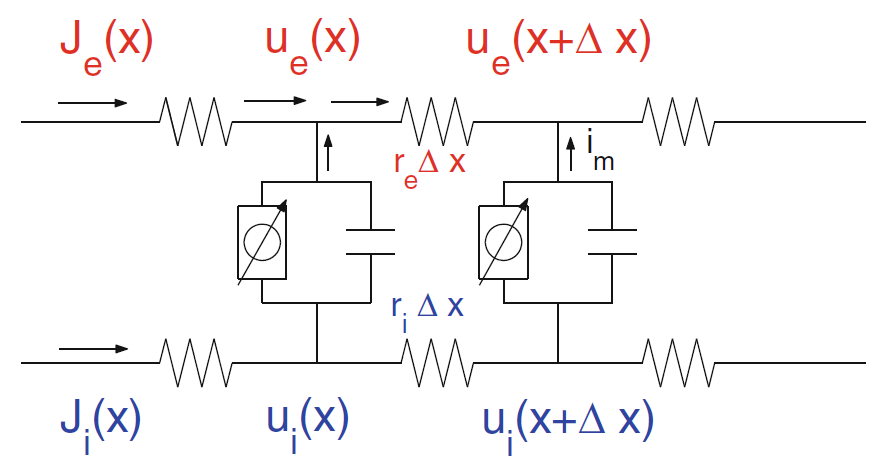
\includegraphics[scale=.35]{fig/cable_model}
\caption{Bi-domain model squeme.} \label{fig:bidomain_model}
\end{figure}

\textbf{PP-formulation:} Let us define the intern and extra cellular conductive tensors $D_i$ and $D_e$, respectively. Given the applied intra and extracellular currents per units volume $I_{i,e}^s: \Omega \times (0,T) \rightarrow \mathbb{R}$, and initial conditions $v_0 : \Omega \rightarrow \mathbb{R}$, $w_0: \Omega \rightarrow \mathbb{R}^k$, $z_0: \Omega \rightarrow (0, +\infty)^m$, find the intra and extracellular potentials $u_{i,e}:\Omega \times (0,T) \rightarrow \mathbb{R}^k$ and the ionic concentrations variables $\vec{r}: \Omega \times (0,T) \rightarrow \mathbb{R}^m$ such that:

\begin{equation}
\arraycolsep=1.4pt\def\arraystretch{2.2}
\begin{array}{rlr}
c_m \dfrac{\partial v}{\partial t} - div(D_i \nabla u_i) + I_{ion}(u_{i,e}, \vec{r}) &= I_{i}^s & \text{ in } \Omega \times (0,T) \\
-c_m \dfrac{\partial v}{\partial t } - div(D_e \nabla u_e) - I_{ion}(u_{i,e}, \vec{r}) &= I_e^s & \text{ in }\Omega \times (0,T) \\
\end{array}
\label{eq:BDM}
\end{equation}

The reaction term $I_{ion}$ and the ODE system for the gating variables are given by the cellular membrane electrical activity model. 

\subsubsection{The Mono Domain Model}

The bi-domain model is highly computational expensive because of the involvement of different space and time scales. Indeed, a complete heartbeat can last nearly 1 second, while the time constants of the rapid kinetics involved ranges from 0.1 to 500 ms. For the space scale, are involved portions of cardiac tissue of the order of centimeters, while the electric potential propagates trough layers of the order of a tenth of a millimeter.

Since the above, usually the \textsl{mono-domain model} equations are solved for large domains, which are a simplification of the bi-domain model. Let us define the following:

\begin{itemize}
\item The scaled transmembrane potential $\phi: \Omega \times \mathbb{R^+}$.
\item The conductivity tensor $D \in \mathbb{R}^{d \times d}$.
\end{itemize}

The mono-domain model can be written as follows:

\begin{equation}
\arraycolsep=1.4pt\def\arraystretch{2.2}
\begin{array}{rl}
\dfrac{\partial \phi}{ \partial t} - div(D \nabla \phi) &= I_{ion} (\phi, \vec{r}) \\
\end{array}
\label{eq:MDE}
\end{equation}

The interpretation of $I_{ion} (\phi, \vec{r})$ is subjected to the choice of the cell electrical activity model. Also note that the Fick's first diffusion law has been adopted.

Finally, in order to reproduce the cardiac tissue properties from a macroscopic point of view, the diffusion tensor is often taken as follows:

\begin{equation}
D = d_1 \hat{f} \otimes \hat{f} + d_2 \hat{c} \otimes \hat{c} \label{eq:macroscopic_diff_tensor}
\end{equation}

where $d_1$ and $d_2$ are the diffusivity for principal and transverse fiber directions, respectively, which are described by unit vectors $\hat{f}$ and $\hat{c}$. The tissue anisotropy will be considered by setting $d_1 = \gamma                                    
d_2$, with $\gamma > 1$. 

\subsection{Cellular Membrane Electrical Activity Models}

\subsubsection{FitzHugh-Nagumo Model}

To describe the source $I_{ion}$, the FitzHugh-Nagumo (FHN) reduced ionic model can be used, which can be written as follows:

\begin{align}
I_{ion}(\phi, w) &= c_1 \phi (\phi - \alpha)(1 - \phi) - c_2 w \\
\dfrac{\partial w}{\partial t} &= c_2 (\phi - wd) \nonumber
\end{align}


where $c_1$, $c_2$ and $d$ are real positive numbers, representing the excitation rate, the excitation decay and the recovery decay of the cell, respectively. Note that we are using the transmembrane potential $\phi$ to write the model, but eventually the FHN equations can be plugged in the bi-domain equations too. In this case, only one recovery variable models the whole membrane electrical activity, therefore the recovery variable vector has only one component, i.e., $\vec{r} = w$.


\subsubsection{Minimal Ventricular Model} 

Other accepted model for the membrane electrical activity is the so called \textsl{Minimal Model} proposed by Bueno-Orovio \cite{BUENO_OROVIO_MINIMAL}. This model takes in account three gating variables, let say $\vec{r} = (r,w,s)$, and can be written as follows:

\begin{equation}
\arraycolsep=1.4pt\def\arraystretch{1.5}
\begin{array}{lr}
I_{ion}(\phi, r, w, s) = - (J_{fi} + J_{so} + J_{si}) \\ 
\partial_t r = (1 - H(\phi - \theta_v))(r_\infty - r)/\tau_{v}^- - H(\phi - \theta_v)r/\tau_v^+ \\
\partial_t w = (1 - H(\phi - \theta_w))(w_\infty - w)/\tau_{w}^- - H(\phi - \theta_w)w/\tau_w^+ \\
\partial_t s = ((1 + tanh(k_s(\phi - \phi_s)))/2 - s)/\tau_s
\end{array} \label{eq:mde_min}
\end{equation}

where $H:\mathbb{R} \rightarrow \mathbb{R}$ is the heaviside function, defined by:

\begin{equation}
\arraycolsep=1.4pt\def\arraystretch{1.5}
H(x) = 
\left\lbrace
\begin{array}{lr}
1 & if~~x > 0 \\
0 & if~~x \leq 0
\end{array} 
\right. \label{eq:HS}
\end{equation}

and where,

\begin{equation}
\arraycolsep=1.4pt\def\arraystretch{1.5}
\begin{array}{lr}
J_{fi} = -r H(\phi - \theta_r)(\phi - \theta_r)(\phi_u - \phi)/ \tau_{fi} \\
J_{so} = (\phi - \phi_0)(1 - H(\phi - \theta_w))/\tau_o + H(\phi - \theta_w)/\tau_{so} \\
J_{si} = -H(\phi - \theta_w)ws/\tau_{si} 
\end{array} \label{eq:mde_currents}
\end{equation}

are the trans-membrane currents considered (fast inward, slow inward and slow outward). It has been shown that this variables retain enough information about cardiac excitation to reproduce exact AP morphologies. This last plus the three gating variables allows to model an action potential that can reproduce arbitrary action potential duration (APD) and conduction velocity (CV) restitution curves.

Also, the Bueno-Orovio model needs the following definitions:

\begin{equation}
\arraycolsep=1.4pt\def\arraystretch{1.5}
\begin{array}{lr}
\tau_r^- = (1 - H(\phi - \theta_r^-))\tau_{r1}^- + H(\phi - \theta_r^-)\tau_{r2}^- \\
\tau_w^- = \tau_{w1}^- + (\tau_{w2}^- - \tau_{w1}^-)(1 + tanh(k_w^- (\phi- \phi_w^-)))/2 \\
\tau_{so} = \tau_{so1} + (\tau_{so2} - \tau_{so1})(1 + tanh(k_{so}(\phi - \phi_{so})))/2 \\
\tau_s = (1 - H(\phi - \theta_w))\tau_{s1} + H(\phi - \theta_w)\tau_{s2} \\
\tau_0 = (1 - H(\phi - \theta_i)) \tau_{o1} + H(\phi - \theta_o) \tau_{o2} \\
\end{array} \label{eq:mde_parameters}
\end{equation}

and,

\begin{equation}
r_{\infty} = \left\lbrace \begin{array}{cr}
1 & \phi < \theta_r^- \\
0 & \phi \geqslant \theta_r^-
\end{array} \right.
~~~~~~~~w_{\infty} = (1 - H(\phi - \theta_o))(1 - \phi/\tau_{w\infty}) + H(\phi - \theta_o)w_{\infty}^*
\end{equation}


For remain parameters see table \ref{tab:parametros_minimal}, where four sets of values are shown for different layers of the  hearth's wall, i.e., for epicardium (EPI), mid-myocardial (MID), epicardial (EPI) and for the atrial tissue. Parameters were taken from Bueno-Orovio results in \cite{BUENO_OROVIO_MINIMAL} and \cite{MINIMAL_ATRIAL}. 


% Please add the following required packages to your document preamble:
% \usepackage{booktabs}
\begin{table}[H]
	\centering
	\caption{Four different set of parameters for cell Minimal Model.}
	\label{tab:parametros_minimal}
	\begin{tabular}{@{}cccccc@{}}
		\toprule
		id & Parameter     & EPI    & ENDO   & MID    & ATRIAL \\ \midrule
		1  & $\phi_0$      & 0      &        & 0      & 0      \\
		2  & $\phi_u$      & 1.55   & 1.56   & 1.61   & 1.02   \\
		3  & $\theta_r$    & 0.3    & 0.3    & 0.3    & 0.302  \\
		4  & $\theta_w$    & 0.13   & 0.13   & 0.13   & 0.33   \\
		5  & $\theta_r^-$  & 0.006  & 0.2    & 0.1    & 0.172  \\
		6  & $\theta_0$    & 0.006  & 0.006  & 0.005  & 0.06   \\
		7  & $\tau_{r1}^-$ & 60     & 75     & 80     & 65.6   \\
		8  & $\tau_{r2}^-$ & 1150   & 10     & 1.4506 & 1150   \\
		9  & $\tau_r^+$    & 1.4506 & 1.4506 & 1.4506 & 0.95   \\
		10 & $\tau_{w1}^-$ & 60     & 6      & 70     & 170.8  \\
		11 & $\tau_{w2}^-$ & 15     & 140    & 8      & 112.4  \\
		12 & $k_w^-$       & 65     & 200    & 200    & 135    \\
		13 & $\phi_w^-$    & 0.03   & 0.016  & 0.016  & 0.744  \\
		14 & $\tau_w^+$    & 200    & 280    & 280    & 217    \\
		15 & $\tau_{fi}$   & 0.11   & 0.1    & 0.078  & 0.0678 \\ 
		16 & $\tau_{o1}$       & 400     & 470    & 410 & 100   \\
		17 & $\tau_{o2}$       & 6       & 6      & 7 & 64.87     \\
		18 & $\tau_{so1}$      & 30.0181 & 40     & 91 & 53.54    \\
		19 & $\tau_{so2}$      & 0.9957  & 1.2    & 0.8 & 8.03   \\
		20 & $k_{so}$          & 2.0458  & 2      & 2.1 & 1.748   \\
		21 & $\phi_{so}$       & 0.65    & 0.65   & 0.6 & 0.644   \\
		22 & $\tau_{s1}$       & 2.7342  & 2.7342 & 2.7342 & 5.406 \\
		23 & $\tau_{s2}$       & 16      & 2      & 4 & 52.91     \\
		24 & $k_s$             & 2.0994  & 2.0994 & 2.0994 & 1.008 \\
		25 & $\phi_s$          & 0.9087  & 0.9087 & 0.9087 & 0.814 \\
		26 & $\tau_{si}$       & 1.8875  & 1.9013 & 3.3849 & 6.978 \\
		27 & $\tau_{w \infty}$ & 0.07    & 0.0273 & 0.01 & 4.97  \\
		28 & $w_{\infty}$         & 0.94    & 0.78   & 0.5 & 1   \\ \hline
\end{tabular}
\end{table}


\subsection{Homogenization}

Due to the multiscale nature of the problem, the application of some results from the Homogenization theory \cite{homogenization} can improve the computational performance in coarse meshes still preserving the influence of the mesoscopic configuration into the macroscopic scale.

\subsubsection{Homogenization Theorem for Diffusion Equations}

\subsubsection*{Rank 1 Laminations}

First, we gonna verify a homogenization theorem for a static diffusion problem over a domain with two materials, where one of them is laminated over the other, in order to eventually expand the theorem beyond his boundaries (where has no formal proof, as the case with a reaction term). So, let us consider two materials, $d_1$ and $d_2$, with $D_1$ and $D_2$ constant diffusion tensors, respectively. Also, let us define $\theta \in \mathbb{R}$ the proportion of the material $D_1$ over the rest of the domain and $e_1 \in \mathbb{R}^d$ the lamination direction (see Figure \ref{fig:lamination_fig}), which is orthogonal to the fiber direction.

Homogenization theory has been a very succesfull mathematical theory dealing with linear difussion equations (and many other systems). However, up to the knowledge of the authors, there are no newer results to be directly applied to the nonlinear and coupled system described, e.g., in \ref{eq:mde_min}. Nevertheless, we propose to apply, as a linear approximation to the full nonlinear homogenization system, the following surrogate model for the effective diffusion tensor:

\begin{equation}
D^{eff} = \theta D_1 + (1 - \theta) D_2 - \frac{\theta (1 - \theta)(D_1 - D_2)e_1 \otimes (D_1 - D_2)^T e_1}{(1 - \theta)D_1 e_1 \cdot e_1 + \theta D_2 e_1 \cdot e_1 } \label{eq:homogenization_rank1}
\end{equation}

This formula was first obtained by Murat and Tartar in 1978 and applies to linear difussion. We claim that nonlinear effects, eventhough they were not originally considered within these calculations, should not significantly affect the full effective tensor (if exists) by assuming that $I_{ion}$ is bounded in proper functional settings and since the nonlinearities studied here do not include derivatives. Once accepted this surrogate model (indistinctly called homogenized model), one can easily go further by applying sequential laminations as in the sequel.

\begin{figure}[!htbp]
\centering
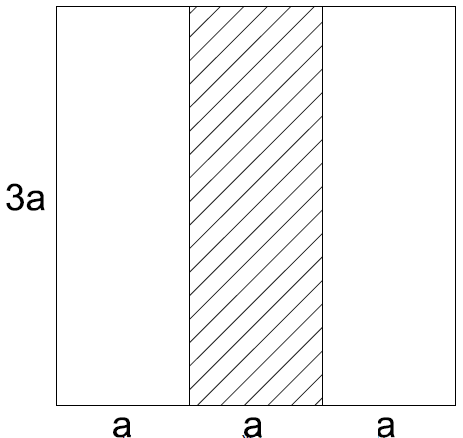
\includegraphics[height = 5 cm]{fig/theorem_verification_r1-ejemplo_laminaciones} 
\caption{Example of a domain with two materials. In this case, the proportion is $\theta = 1/3$ and lamination direction $e_1 = (1,0,0)$.} \label{fig:lamination_fig}
\end{figure}

\subsubsection*{Rank 2 Laminations}

Since in the heart, a more realistic configuration must also consider that healthy cells are slightly separated by collagen, the lamination formula can be repeated once again to reproduce such characteristical pattern (see Figure \ref{fig:geometry_convention}):

\begin{figure}[!htbp]
\centering
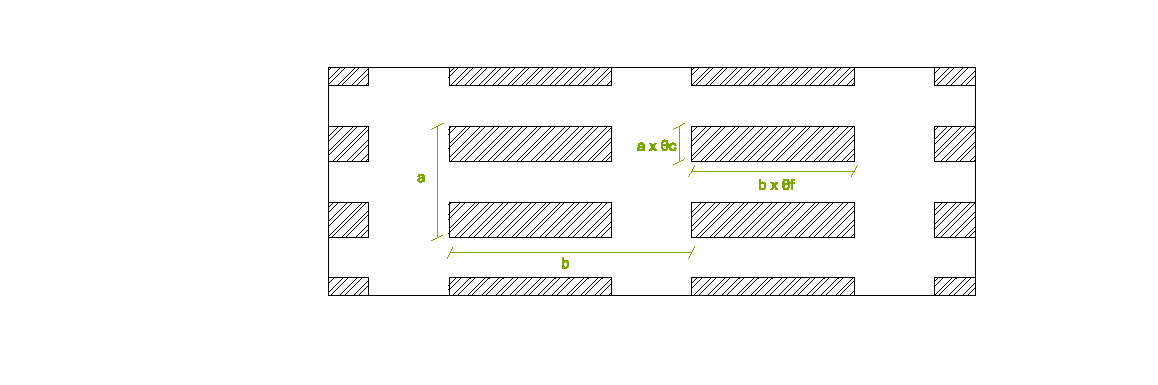
\includegraphics[height = 5 cm]{fig/theorem_verification_r2-geometry_convention} 
\caption{Geometric configuration of the mesoscopic scale of the heart tissue.} \label{fig:geometry_convention}
\end{figure}

Let us consider two laminations directions defined by the local basis $e_1$ and $e_2$, and a collagen diffusion tensor defined as $D_{col} = d_{col} I_{2 \times 2}$, where $d_{col}$ is the collagen diffusivity. Also, let us consider a domain with only collagen within, and the laminations of healthy tissue described by $\hat{f}$ with direction $e_1$. The effective tensor for this configuration will be, according with \ref{eq:homogenization_rank1}:

\begin{equation}
D_{eff}'=
(1 - \theta_c)D_h + \theta_c D_{col} - \frac{\theta_c (1 - \theta_c)(D_{col} - D_{h})e_1 \otimes (D_{col} - D_{h})^T e_1}{(1 - \theta_c)D_{col} e_1 \cdot e_1 + \theta_c D_{h} e_1 \cdot e_1 }
\end{equation}

Having this, we can proceed to laminate with healthy tissue in the cross direction, considerering now an array of laminations described by $\hat{c}$ (with lamination direction $e_2$) inside a domain with a diffusion tensor $D_{eff}'$. So that, if $D_{eff}$ is the effective diffusion tensor for the domain with the two array of laminations, we can write:

\begin{equation}
D_{eff} = 
(1 - \theta_f)D_h + \theta_f D_{eff}' - \frac{\theta_f (1 - \theta_f)(D_{eff}' - D_h)e_2 \otimes (D_{eff}' - D_h)^T e_2}{(1 - \theta_f)D_{eff}' e_2 \cdot e_2 + \theta_f D_h e_2 \cdot e_2 }
\end{equation}